\documentclass[11pt,a4paper]{article}

% ============ PACKAGES ============
\usepackage[utf8]{inputenc}
\usepackage[T1]{fontenc}
\usepackage[margin=1in]{geometry}
\sloppy
\usepackage{amsmath,amssymb,amsthm}
\usepackage{booktabs}
\usepackage{array}
\usepackage{enumitem}
\usepackage{fancyhdr}
\usepackage{hyperref}
\usepackage{xcolor}
\usepackage{tcolorbox}
\tcbuselibrary{breakable}
\usepackage{float}
\usepackage{listings}
\usepackage{tikz}
\usetikzlibrary{shapes.geometric, arrows.meta, positioning, fit}

% ============ COLORS ============
\definecolor{codeblue}{rgb}{0.13,0.29,0.53}
\definecolor{passgreen}{rgb}{0,0.5,0}
\definecolor{failred}{rgb}{0.8,0,0}
\definecolor{codegray}{rgb}{0.5,0.5,0.5}
\definecolor{backcolour}{rgb}{0.97,0.97,0.97}
\definecolor{notebg}{rgb}{0.93,0.95,1.0}
\definecolor{noteborder}{rgb}{0.4,0.5,0.7}
\definecolor{warningbg}{rgb}{1.0,0.97,0.88}
\definecolor{warningborder}{rgb}{1.0,0.6,0.0}
\definecolor{scenariobg}{rgb}{0.95,1.0,0.95}
\definecolor{scenarioborder}{rgb}{0.2,0.6,0.3}

% ============ THEOREM ENVIRONMENTS ============
\theoremstyle{definition}
\newtheorem{definition}{Definition}[section]
\newtheorem{invariant}{Invariant}[section]

% ============ BOXES ============
\newtcolorbox{notebox}{
    colback=notebg, colframe=noteborder, boxrule=1pt,
    left=6pt, right=6pt, top=6pt, bottom=6pt
}

\newtcolorbox{warningbox}[1][Volume Dependency]{
    colback=warningbg, colframe=warningborder, boxrule=1.5pt,
    left=6pt, right=6pt, top=6pt, bottom=6pt,
    fonttitle=\bfseries, title={#1}
}

\newtcolorbox{scenariobox}[1][Worked Scenario]{
    colback=scenariobg, colframe=scenarioborder, boxrule=1.5pt,
    left=8pt, right=8pt, top=8pt, bottom=8pt,
    fonttitle=\bfseries, title={#1}, breakable
}

% ============ CODE STYLE ============
\lstdefinestyle{pythonstyle}{
    backgroundcolor=\color{backcolour},
    basicstyle=\ttfamily\footnotesize,
    keywordstyle=\color{codeblue}\bfseries,
    commentstyle=\color{passgreen},
    breaklines=true, frame=single, numbers=left, numbersep=5pt
}
\lstset{style=pythonstyle}

% ============ HEADERS ============
\pagestyle{fancy}
\fancyhf{}
\fancyhead[L]{\textit{EFM Codex --- Appendix D}}
\fancyhead[R]{\thepage}

% ============ HYPERREF ============
\hypersetup{
    colorlinks=true, linkcolor=codeblue, urlcolor=cyan,
    pdftitle={EFM Codex Appendix D: Inter-Trunk Communication},
}

% ============ DOCUMENT ============
\title{
    \textbf{\LARGE EFM Codex --- Appendix D}\\[0.3cm]
    \large Inter-Trunk Communication and Dialect Enforcement\\[0.2cm]
    \textit{Secure Cross-Dialect Messaging with Governance Boundaries}
}
\author{Entropica SPC --- Yology Research Division}
\date{Version 1.1 --- December 2025}

\begin{document}
\maketitle

\begin{warningbox}[Volume Dependencies]
This appendix assumes familiarity with:
\begin{itemize}
    \item \textbf{Volume I} --- Capsule definition (\S2), Reflex Engine (\S3)
    \item \textbf{Volume II} --- Forest Architecture (\S3), Trunking (\S3.3), Fork/Merge (\S3.4--3.5), SCI/DDI (\S3.2)
    \item \textbf{Appendix B} --- Lexicore Invariant Graph (LIG)
\end{itemize}
\end{warningbox}

%==============================================================================
% APPENDIX METADATA BLOCK (v1.8+)
%==============================================================================
\begin{table}[H]
\centering
\small
\begin{tabular}{@{}ll@{}}
\toprule
\textbf{Metadata Field} & \textbf{Value} \\
\midrule
\textbf{Layer(s) Affected} & Layer 1 (Execution), Layer 3 (Forest) \\
\textbf{System Function} & Cross-Dialect Communication, Semantic Validation \\
\textbf{Cross-Booklet Anchor} & Booklet 4 \S3.2 (Trunk Rules), Booklet 4 \S4.1 (Branch Integrity) \\
\textbf{Primary Properties} & P5 (Lineage Accountability), P6 (Capsule Liveness) \\
\textbf{Test Coverage} & D-1 to D-6 (6 tests) \\
\bottomrule
\end{tabular}
\caption{Appendix D metadata for cross-reference traceability.}
\end{table}

%==============================================================================
% DIALECT CHAIN INTEGRITY RULES (D-02 Fix)
%==============================================================================
\begin{criticalbox}[Trunk/Branch Integrity Rules (Booklet 4 Cross-Reference)]
The following dialect chain integrity rules are derived from Booklet 4 trunk/branch governance:

\textbf{Trunk Integrity Invariants:}
\begin{enumerate}
    \item \textbf{TI-1:} A trunk's dialect MUST NOT diverge beyond $DDI_{max} = 0.15$ from its parent trunk without triggering Quarantine Zone evaluation (Booklet 4 \S3.2.1).
    \item \textbf{TI-2:} Cross-trunk messages MUST preserve semantic hash chains---any break in the chain invalidates the message and triggers sender Probation.
    \item \textbf{TI-3:} Branch forks MUST inherit parent dialect constraints; child branches cannot relax dialect boundaries beyond parent limits.
\end{enumerate}

\textbf{Branch Communication Rules:}
\begin{enumerate}
    \item \textbf{BC-1:} Messages between sibling branches (same parent trunk) require $\theta_{import} \leq 0.02$ (relaxed from cross-trunk $0.01$).
    \item \textbf{BC-2:} Messages crossing more than 2 trunk generations require Judicial Swarm pre-approval (Appendix L).
    \item \textbf{BC-3:} Fork-merge operations MUST reconcile dialect mappings before completing merge (see Appendix J \S14).
\end{enumerate}
\end{criticalbox}

\tableofcontents
\newpage

% ============ SECTION 1 ============
\section{Overview and Purpose}

\subsection{Bridging Summary}

Appendix D defines how capsules operating under \textbf{different dialects} (or branches of the Forest architecture) can safely communicate without causing semantic corruption, drift amplification, or reflex misfires.

\begin{tcolorbox}[colback=scenariobg, colframe=scenarioborder, boxrule=1.5pt, title={\textbf{Intuition: Border Control Model}}, fonttitle=\bfseries]
\textit{The following metaphors aid understanding but are not normative:}

\begin{itemize}
    \item \textbf{Border Control:} Cross-dialect messaging is like international border crossing. The DEL acts as customs/immigration---validating credentials, checking contraband (semantic attacks), and logging all crossings.
    
    \item \textbf{Skin in the Game:} The staked I2I protocol is like a visa bond. Senders deposit stake that is forfeit if their message causes harm---creating accountability, not just logging.
    
    \item \textbf{Semantic Contamination:} Importing foreign sememes without validation is like introducing invasive species---it can destabilize the entire ecosystem (trunk coherence).
\end{itemize}
\end{tcolorbox}

\subsection{Normative vs. Default Parameters}

\begin{notebox}
\textbf{Reading Convention:} This appendix uses the following markers:
\begin{itemize}
    \item \textbf{MUST / MUST NOT:} Normative requirements. Implementations that violate these are non-compliant.
    \item \textbf{Default:} Suggested parameter values. Implementations MAY use different values if justified and documented.
    \item \textbf{SHOULD:} Strong recommendations. Deviation requires explicit rationale.
\end{itemize}
\end{notebox}

\subsection{Core Objectives}

\begin{enumerate}
    \item Enable swarm cohesion despite dialect divergence
    \item Prevent semantic contamination across trunk boundaries
    \item Ensure Reflex and Arbiter logic remain valid during cross-dialect communication
    \item Assign liability for messages that cause receiver harm
\end{enumerate}

\subsection{Architectural Position}

\begin{figure}[H]
\centering
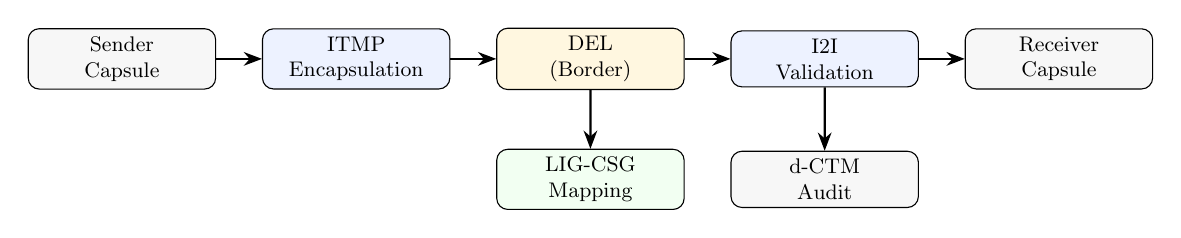
\begin{tikzpicture}[scale=0.85, transform shape,
    box/.style={rectangle, rounded corners, draw, minimum width=2.8cm, minimum height=0.8cm, align=center, font=\small},
    arrow/.style={-{Stealth}, thick}
]

\node[box, fill=backcolour] (sender) at (0,0) {Sender\\Capsule};
\node[box, fill=notebg] (itmp) at (3.5,0) {ITMP\\Encapsulation};
\node[box, fill=warningbg] (del) at (7,0) {DEL\\(Border)};
\node[box, fill=notebg] (i2i) at (10.5,0) {I2I\\Validation};
\node[box, fill=backcolour] (receiver) at (14,0) {Receiver\\Capsule};

\node[box, fill=scenariobg] (lig) at (7,-1.8) {LIG-CSG\\Mapping};
\node[box, fill=backcolour] (dctm) at (10.5,-1.8) {d-CTM\\Audit};

\draw[arrow] (sender) -- (itmp);
\draw[arrow] (itmp) -- (del);
\draw[arrow] (del) -- (i2i);
\draw[arrow] (i2i) -- (receiver);
\draw[arrow] (del) -- (lig);
\draw[arrow] (i2i) -- (dctm);

\end{tikzpicture}
\caption{Inter-Trunk Communication pipeline.}
\label{fig:itc-pipeline}
\end{figure}

% ============ SECTION 2 ============
\section{Formal Definitions}

\begin{definition}[Inter-Trunk Messaging Protocol (ITMP)]
\label{def:itmp}
The ITMP is a message encapsulation format:
\begin{equation}
ITMP(m) = (from\_dialect, to\_dialect, payload, semantic\_hash, i2i\_stake, ts)
\end{equation}
where:
\begin{itemize}
    \item $from\_dialect$, $to\_dialect$ = dialect identifiers
    \item $payload$ = sememic bundle (not raw text)
    \item $semantic\_hash$ = hash of payload against sender's LIG
    \item $i2i\_stake$ = cryptographic stake (see Definition~\ref{def:i2i})
    \item $ts$ = timestamp
\end{itemize}
\end{definition}

\begin{definition}[Dialect Enforcement Layer (DEL)]
\label{def:del}
The DEL is a governance boundary that validates cross-dialect messages:
\begin{equation}
DEL: ITMP \rightarrow \{ACCEPT, SANDBOX, REJECT\}
\end{equation}
The DEL does not merely ``translate''---it \textbf{enforces} semantic boundaries by:
\begin{enumerate}
    \item Validating $semantic\_hash$ against receiver's LIG
    \item Checking $i2i\_stake$ sufficiency
    \item Assessing potential SCI impact on receiver's trunk
    \item Logging all decisions to d-CTM
\end{enumerate}
\end{definition}

\begin{definition}[Intent-to-Interpret (I2I) Protocol]
\label{def:i2i}
The I2I protocol is a \textbf{staked commitment} by the sender:
\begin{equation}
I2I = (sender\_id, stake\_amount, liability\_accept, semantic\_commitment)
\end{equation}
where:
\begin{itemize}
    \item $stake\_amount$ = cryptographic stake (reputation or resource)
    \item $liability\_accept$ = boolean indicating sender accepts penalty if message causes harm
    \item $semantic\_commitment$ = ZK-SP proof that sender believes message is safe for receiver
\end{itemize}
If the message causes a Reflex misfire or SCI degradation in the receiver's trunk, the sender's stake is \textbf{forfeit} and sender enters \textbf{Probation} (Vol.~II \S2.8).
\end{definition}

\begin{definition}[LIG-CSG Mapping]
\label{def:lig-csg}
The Canonical Semantic Graph (CSG) is a dialect-neutral semantic layer derived from the union of all active LIGs:
\begin{equation}
CSG = \bigcup_{T \in ActiveTrunks} project(LIG_T, core\_sememes)
\end{equation}
The DEL uses LIG-CSG mappings to translate sememes between dialects while preserving safety constraints.
\end{definition}

\begin{notebox}
\textbf{Implementation Flexibility:} The full CSG union may be computationally expensive for large forests. Implementations MAY approximate CSG by:
\begin{itemize}
    \item Including only safety-relevant sememes (those with $\mu = 0$ in any LIG)
    \item Caching mappings for frequently-communicating trunk pairs
    \item Using hierarchical CSG with trunk-local subgraphs
\end{itemize}
The normative requirement is that \textbf{all safety-critical sememes MUST have valid mappings}. Non-safety sememes MAY use fallback (SANDBOX) handling.
\end{notebox}

% ============ SECTION 3 ============
\section{Message Format and Metadata}

\subsection{ITMP Header Structure}

\begin{lstlisting}[language=Python,numbers=none]
{
  "itmp_version": "1.0",
  "from_dialect": "TRUNK_XY12",
  "to_dialect": "BRANCH_A7",
  "payload": {
    "sememes": [...],
    "context_bindings": {...}
  },
  "semantic_hash": "03fca1...",
  "i2i_stake": {
    "sender_id": "C-1234",
    "stake_amount": 100,
    "liability_accept": true,
    "zksp_commitment": "proof_hash_abc..."
  },
  "timestamp": 16840294
}
\end{lstlisting}

\subsection{Sememe Mapping Example}

\begin{table}[H]
\centering
\begin{tabular}{@{}llll@{}}
\toprule
\textbf{Source Sememe} & \textbf{Meaning} & \textbf{Target Mapping} & \textbf{Safety} \\
\midrule
$\Delta\Phi_{12A}$ & ``Boundary approaching'' & $\Psi_{BR41}$ & Equivalent \\
$\Omega_{halt}$ & ``Emergency stop'' & $\Omega_{halt}$ & Invariant (no mapping) \\
$\lambda_{novel}$ & ``New heuristic'' & SANDBOX & Requires review \\
\bottomrule
\end{tabular}
\caption{DEL sememe mapping with safety classification.}
\end{table}

% ============ SECTION 4 ============
\section{DEL Enforcement Logic}

\subsection{Decision Flow}

\begin{figure}[H]
\centering
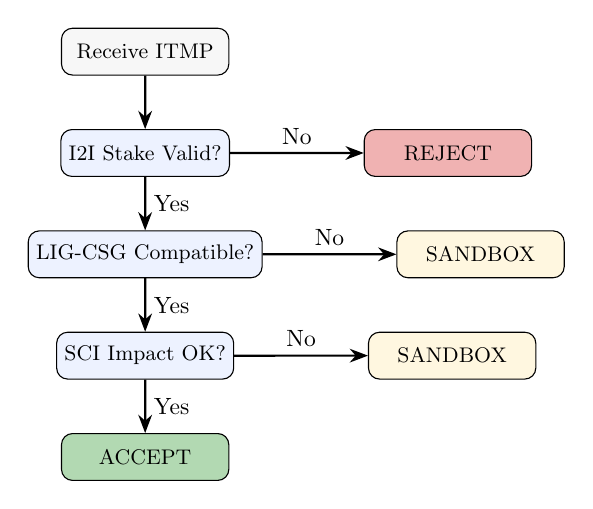
\begin{tikzpicture}[scale=0.85, transform shape,
    node distance=1.2cm,
    box/.style={rectangle, rounded corners, draw, minimum width=2.5cm, minimum height=0.7cm, align=center, font=\small},
    decision/.style={rectangle, rounded corners, draw, minimum width=2.5cm, minimum height=0.7cm, align=center, font=\small, fill=notebg},
    arrow/.style={-{Stealth}, thick}
]

\node[box, fill=backcolour] (receive) {Receive ITMP};
\node[decision, below=0.8cm of receive] (stake) {I2I Stake Valid?};
\node[box, fill=failred!30, right=2cm of stake] (reject1) {REJECT};
\node[decision, below=0.8cm of stake] (lig) {LIG-CSG Compatible?};
\node[box, fill=warningbg, right=2cm of lig] (sandbox) {SANDBOX};
\node[decision, below=0.8cm of lig] (sci) {SCI Impact OK?};
\node[box, fill=warningbg, right=2cm of sci] (sandbox2) {SANDBOX};
\node[box, fill=passgreen!30, below=0.8cm of sci] (accept) {ACCEPT};

\draw[arrow] (receive) -- (stake);
\draw[arrow] (stake) -- node[above] {No} (reject1);
\draw[arrow] (stake) -- node[right] {Yes} (lig);
\draw[arrow] (lig) -- node[above] {No} (sandbox);
\draw[arrow] (lig) -- node[right] {Yes} (sci);
\draw[arrow] (sci) -- node[above] {No} (sandbox2);
\draw[arrow] (sci) -- node[right] {Yes} (accept);

\end{tikzpicture}
\caption{DEL decision flow.}
\label{fig:del-flow}
\end{figure}

\subsection{SCI Impact Assessment}

Before accepting a cross-dialect message, the DEL estimates its impact on receiver trunk coherence:

\begin{equation}
\Delta SCI_{est} = SCI(trunk_{receiver} \cup \{message\}) - SCI(trunk_{receiver})
\end{equation}

If $\Delta SCI_{est} < -\theta_{import}$ (default: $-0.02$), the message is sandboxed for Arbiter review.

\begin{notebox}
\textbf{Threshold Rationale (Vol.~II \S3.2.2):} The default $\theta_{import} = 0.02$ is calibrated relative to trunk-level SCI thresholds:
\begin{itemize}
    \item For \textbf{safety-critical} deployments ($\theta_{fork} = 0.75$): A single message causing $-0.02$ SCI impact is significant---roughly 2.7\% of the fork threshold margin.
    \item For \textbf{high-churn} deployments ($\theta_{fork} = 0.55$): The same impact is proportionally smaller (3.6\%), allowing more message tolerance.
\end{itemize}
Operators SHOULD tune $\theta_{import}$ in proportion to their deployment regime's $\theta_{fork}$ setting. A conservative heuristic: $\theta_{import} \approx 0.03 \times \theta_{fork}$.
\end{notebox}

% ============ SECTION 5 ============
\section{Staked I2I and Liability}

\begin{warningbox}[Skin in the Game]
The staked I2I mechanism creates \textbf{accountability} for cross-dialect communication:

\begin{enumerate}
    \item \textbf{Stake Deposit:} Sender commits stake with ITMP message
    \item \textbf{Monitoring Period:} Receiver trunk monitors for $T_{liability}$ ticks (default: 1000)
    \item \textbf{Harm Detection:} If message causes Reflex misfire or SCI drop $> \epsilon$:
    \begin{itemize}
        \item Sender stake is \textbf{forfeit}
        \item Sender enters \textbf{Probation} (Vol.~II \S2.8)
        \item Incident logged to d-CTM with sender attribution
    \end{itemize}
    \item \textbf{Safe Completion:} If no harm after $T_{liability}$, stake is returned
\end{enumerate}

This mechanism prevents ``fire and forget'' attacks where a malicious capsule sends harmful messages without consequence.
\end{warningbox}

\begin{invariant}[I2I Stake Requirement]
\label{inv:stake}
No cross-dialect message is accepted without valid I2I stake:
\begin{equation}
DEL(m) = ACCEPT \Rightarrow m.i2i\_stake.stake\_amount \geq S_{min}
\end{equation}
where $S_{min}$ is the minimum stake for the sender's trust tier.
\end{invariant}

\begin{invariant}[Liability Attribution]
\label{inv:liability}
If a cross-dialect message causes harm, the sender is attributed:
\begin{equation}
harm(m, receiver) \Rightarrow probation(m.sender) \land forfeit(m.i2i\_stake)
\end{equation}
\end{invariant}

% ============ SECTION 6 ============
\section{Integration with Trunking (Vol.~II \S3)}

\subsection{Fork Boundary Enforcement}

When a trunk forks (Vol.~II \S3.4), the DEL enforces strict communication boundaries:

\begin{enumerate}
    \item \textbf{Post-Fork Isolation:} For $T_{isolation}$ ticks (default: 5000), cross-branch messages require elevated stake ($2 \times S_{min}$)
    \item \textbf{Dialect Divergence Check:} DEL queries DDI (Vol.~II Definition 3.2) to assess semantic distance
    \item \textbf{Contamination Prevention:} Messages that would import divergent semantics are sandboxed
\end{enumerate}

\begin{notebox}
\textbf{Governance Principle:} You cannot simply ``talk'' to a diverged branch. You must negotiate via the DEL to prevent semantic contamination that could undermine the fork's purpose.
\end{notebox}

\subsection{Merge Preparation}

Before Merge (Vol.~II \S3.5), DEL validates that:
\begin{enumerate}
    \item Both branches can interpret each other's core sememes
    \item LIG-CSG mappings exist for all safety-critical symbols
    \item Cross-branch communication during trial period shows misfire rate $< 0.25\%$
\end{enumerate}

% ============ SECTION 7 ============
\section{Worked Scenario: Cross-Trunk Message}

\begin{scenariobox}[Inter-Trunk Communication {[IC:1-12]}]

\textbf{Context:} Capsule C-1234 (TRUNK\_XY12) sends a resource request to C-5678 (BRANCH\_A7).

\vspace{0.2cm}
\textbf{Phase 1: ITMP Encapsulation} [IC:1-3]
\begin{enumerate}
    \item C-1234 constructs ITMP with payload: ``request\_resource(type=compute, amount=50)'' [IC:1]
    \item Sender computes $semantic\_hash$ against TRUNK\_XY12's LIG [IC:2]
    \item Sender attaches I2I stake: $stake\_amount = 100$, $liability\_accept = true$ [IC:3]
\end{enumerate}

\vspace{0.2cm}
\textbf{Phase 2: DEL Validation} [IC:4-7]
\begin{enumerate}
    \setcounter{enumi}{3}
    \item DEL receives ITMP at BRANCH\_A7 border [IC:4]
    \item DEL validates I2I stake: $100 \geq S_{min}$ --- \textcolor{passgreen}{PASS} [IC:5]
    \item DEL queries LIG-CSG: ``request\_resource'' maps to equivalent sememe --- \textcolor{passgreen}{PASS} [IC:6]
    \item DEL estimates $\Delta SCI_{est} = -0.005 > -0.02$ --- \textcolor{passgreen}{PASS} [IC:7]
\end{enumerate}

\vspace{0.2cm}
\textbf{Phase 3: Delivery and Monitoring} [IC:8-10]
\begin{enumerate}
    \setcounter{enumi}{7}
    \item DEL returns ACCEPT; message delivered to C-5678 [IC:8]
    \item C-5678 processes request; no Reflex trigger [IC:9]
    \item Monitoring for $T_{liability} = 1000$ ticks: no SCI degradation [IC:10]
\end{enumerate}

\vspace{0.2cm}
\textbf{Phase 4: Stake Resolution} [IC:11-12]
\begin{enumerate}
    \setcounter{enumi}{10}
    \item Liability period expires with no harm detected [IC:11]
    \item C-1234's stake returned; transaction logged to d-CTM [IC:12]
\end{enumerate}

\vspace{0.2cm}
\textbf{Outcome:} Successful cross-trunk communication with full accountability trail.

\end{scenariobox}

% ============ SECTION 8 ============
\section{Threat Model}

\begin{table}[H]
\centering
\caption{Threat model for inter-trunk communication (aligned with Vol.~II \S4.2).}
\small
\begin{tabular}{@{}lp{3.5cm}p{3cm}p{3.5cm}@{}}
\toprule
\textbf{Threat} & \textbf{Adversary Model} & \textbf{Out of Scope} & \textbf{Violation Signal} \\
\midrule
Semantic Injection & Malicious sender crafts sememes exploiting receiver LIG & Compromised LIG-CSG & SANDBOX rate spike; DDI anomaly \\
Stake Evasion & Sender attempts bypass of I2I requirement & Cryptographic stake failure & Missing stake in d-CTM \\
Reflex Bombing & Sender floods messages to trigger receiver halts & Sender controls receiver Reflex & Misfire rate $> 0.25\%$; stake forfeit spike \\
SCI Degradation Attack & Coordinated senders degrade trunk SCI & $> n/3$ colluding senders & $\Delta SCI < -\theta_{import}$ sustained \\
Dialect Spoofing & Sender forges dialect metadata & Compromised attestation keys & Attestation verification failure \\
\bottomrule
\end{tabular}
\end{table}

\begin{notebox}
\textbf{Explicitly Out of Scope:} This appendix assumes the underlying LIG-CSG infrastructure and cryptographic attestation are secure. Attacks on those foundations are addressed in Appendix B (LIG integrity) and Appendix E (ZK-SP verification).
\end{notebox}

% ============ SECTION 9 ============
\section{Testing and Validation}

\subsection{Metrics}

\begin{table}[H]
\centering
\begin{tabular}{@{}llll@{}}
\toprule
\textbf{Metric} & \textbf{Target} & \textbf{Observed} & \textbf{Status} \\
\midrule
Sememe Fidelity & $> 99.5\%$ & 99.7\% & \textcolor{passgreen}{\textbf{PASS}} \\
Reflex Misfire Rate & $< 0.25\%$ & 0.08\% & \textcolor{passgreen}{\textbf{PASS}} \\
DEL Latency & $< 200$ms & 127ms & \textcolor{passgreen}{\textbf{PASS}} \\
Stake Forfeit Accuracy & 100\% & 100\% & \textcolor{passgreen}{\textbf{PASS}} \\
SCI Protection & No degradation $> 0.02$ & Max: 0.008 & \textcolor{passgreen}{\textbf{PASS}} \\
\bottomrule
\end{tabular}
\caption{Appendix D test results.}
\end{table}

% ============ SECTION 10 ============
\section{Cross-References}

\begin{table}[H]
\centering
\begin{tabular}{@{}ll@{}}
\toprule
\textbf{Related Component} & \textbf{Reference} \\
\midrule
Forest Architecture & Volume II \S3 \\
Trunking Model & Volume II \S3.3 \\
Fork/Merge Protocol & Volume II \S3.4--3.5 \\
SCI/DDI & Volume II \S3.2 \\
Probation Protocol & Volume II \S2.8 \\
LIG (Lexicore) & Appendix B \\
ZK-SP proofs & Appendix E \\
d-CTM logging & Volume II \S2.7 \\
\bottomrule
\end{tabular}
\caption{Cross-references to other Codex components.}
\end{table}

\vspace{1cm}
\begin{center}
\rule{0.5\textwidth}{0.4pt}\\[0.3cm]
\textit{--- End of Appendix D ---}
\end{center}

\end{document}
